\chapter{Describing Machine Learning Approaches} \label{sec:sectionFour}

\section{Machine Learning} \label{sec:machineLearning}

Machine learning has become a popular topic in recent years as an answer to the sheer amount of data that has the potential to be processed.  Not only does the large amount of data require more advanced and intelligent ways to process it, but there is also a big incentives driving the desire to do so.  Through machine learning techniques and patterns additional meaning can be extracted from the data which can be used to draw conclusions or predictions. \cite{dataManagementSystems}  Machine learning techniques are commonly applied to data mining tasks, examining at data and discerning additional information from it.  In the case of this research's problem area the data being mined is the large amount of web requests.

This brings numerous benefits to a security application such as web threat detection, primarily it allows the system to have some sort of feedback mechanicism to improve its detection and perhaps even it's prevention.  A system that is unable to learn overtime will not be able to overcome new techniques designed by attackers to evade the current detection systems abilities unless it is manually updated.  And as discussed before, manual updating is not only a very inefficient time consuming task but it is also just plain infeasible as the number and complexity of these attacks grows.  Identifying patterns from data is very useful when it's consider that many attacks follow some kind of a basic syntax or format and while there are many ways to evade detection, typically there is still a common method or intent that can be identified.

The way machine learning operates is by identifying a series of features in the data set in question, these features are then used by the algorithm learn and make better decisions.  The key distinction of machine learning is that the algorithms are not told what to do explicitly but instead is allowed to make its decision based on measurements such as performance. \cite{supervisedMachineLearning}
  
\subsection{Supervised Learning} \label{sec:supervisedLearning}

Machine learning algorithms can either make use of supervised learning or unsupervised learning.  In supervised learning the system is provided with labelled data, data that states what the end result should be so that the system can be accurately trained without additional intervention.  There is also another type of learning called reinforcement learning where an external source informs the system how well it is working or not as it progresses.

Supervised learning has issues that must to be overcome however, the first of which being collecting the original data set.  If there is prior research or people in the know that can suggest what features to use, then the process is much more trivial, otherwise the features are often identified using a brute force method.  The problem with using a brute force method other than the computation time is that the data has the potential to be noisy and miss important features which can lead to further problems.  Learning from extremely large datasets is very inefficient as well.  Therefore it is often desired to minimize the  size of the data set while still maintaining the final performance of the system through a process is called instance selection.  Lastly, having a large amount of features in the data set can also increase the complexity of the system.  To solve this irrelevant and redundant features should be removed whenever possible, but if many of the features depend on each other then they shouldn't be removed as this can lead to inaccuracies in of the learning process.  To deal with features that can't be removed,, new features can be constructed or existing ones altered to be more concise and accurate, improving the entire system as a whole.

One of the big steps in creating a machine learning system is selecting the right algorithm for the dataset, each which their own advantages, disadvantages and times where they are applicable (Section \ref{sec:sectionSeven}). 

\section{Genetic Algorithm} \label{sec:genAlgorithm}

A genetic algorithm is a search-based algorithm that makes use of machine learning in order to locate optimal or near-optimal solutions for a particular problem.  This is what is meant by the term 'search' that is often used to describe this and other algorithms such as local search or simulated annealing, it is not about locating something in a particular data set but rather searching for the best possible answer.  Such algorithms, especially in the case of a genetic algorithm use fitness functions and possibly reward systems to distinguish between a better solution and one that should not be considered going forward. \cite{searchBasedSoftwareEngineering}

As the name suggests, a genetic algorithm mimics how genetic development in the real world works and how species evolve over time.  The algorithm begins with an initial population of individuals, an individual being a possible solution to the problem in question.  Every individual has it's fitness evaluated using some form of calculation tailored to suit the problem at hand; for our purposes for web threat detection the fitness will be evaluated with the following:

\begin{algorithm}[H]
	\setstretch{1.0}
	\centering

	$fitness = (\frac{correct\ detections}{\alpha})\ - (\frac{false\ positives}{\gamma})\ - (\frac{incorrect\ detections}{\beta \cdot 8})$ \\
	
	$\alpha \leftarrow The\ number\ of\ possible\ correct\ detections$ \\
	$\beta \leftarrow The\ number\ of\ possible\ incorrect\ detections$ \\
	$\gamma \leftarrow The\ number\ of\ possible\ false\ positives$ \\
	
	\caption{Fitness algorithm for use in genetic algorithm}
	\label{alg:fitness}
	\\
\end{algorithm}

Correct detections with improve the fitness of a particular individual and the individual is more likely to be selected for genetic operators later on, where as false positives and incorrect detections impact the fitness negatively, with incorrect detections having less of a negative impact than the former.  As an example, if we are looking for SQL injections, every deleted request that is a SQL injection is correct, if instead it isn't an attack at all then it is a false positive and if it is actually a XSS or RFI attack then this is an incorrect detection.

In order for the genetic algorithm to produce a new population it makes use of what are called genetic operators which commonly include performing crossovers and mutations to the individuals.  Two individuals at a time in the population are selected by a selection algorithm and crossed over, there are many ways to perform a crossover but a single-point crossover will be the method used for this research.  A position is selected to perform the crossover, referred to as a locus, for our purposes this refers to selecting a segment, this segment is then swapped with the other selected individual's respective segment to produce two new individuals with unique chromosomes, or in other words different configurations.  This process continues until the algorithm has produced enough new individuals to fill the next population, in addition, at the beginning of this process it is possible to mark some of the top individuals as elite and bring them into the new population unaltered.  Before continuing to the next generation every single allele, or piece of information in each individual has a small chance to be mutated, this is what causes the population to have some sort of diversity.  This entire process then repeats many times, each time being referred to as a generation and by the end of the process there should be a set of individuals that are closer to solving the problem.

\subsection{Current Genetic Algorithm Solutions} \label{sec:currentGenSolutions}

These genetic algorithm techniques have been applied to web threat detection already, one particular paper focused on using variants of an attack to detect network related attacks.  While they may not have directly used a genetic algorithm in their solution, the core idea is very similar to how a genetic algorithm operates with generating different individuals and seeing if they fit a certain criteria.  These exploit variants were used to test signature based detection methods to see if it was possible to evade them and results showed that it was.  This is proof that traditional models for detection cannot be made absolutely perfect and that the using an approach similar to genetic algorithm technniques is worthwhile for atleast evading detection. \cite{testingNetworkBased}

As of recently research has taken this idea and done the opposite, using a genetic algorithm directly to detect web attacks rather than to evade detection.  The genetic algorithm was used to make variants of attack detection signatures that can best detect SQL injections, XSS, and RFI attacks through the text-based web request logs.  The results of which were very promising with around a 90\% detection accuracy reported which exceeded the performance of a traditional regular expression signature based detection system. \cite{mainPaper}

These recent findings are the starting point for this research, improving the genetic algorithm approach and gathering more detailed results about it's function and performance, as well as being the comparison point for another machine learning technique, support vector machines.

\section{Support Vector Machine} \label{sec:SVM}

A support vector machine's main technique for classifying data is to divide the data set into two or more categories with the largest margin possible between the seperation(s), referred to as a hyperplane(s).  The reason for maximizing this buffer between categories is to reduce the chances of classification error as much as possible.  With the hyperplane(s) computed, points that lie within the margin are referred to as support vectors, hence the name, and it is these points which were used to calculate the hyperplane(s) in the first place with the other data points being ignored (Figure \ref{fig:svmmargin}).  

\begin{figure}
	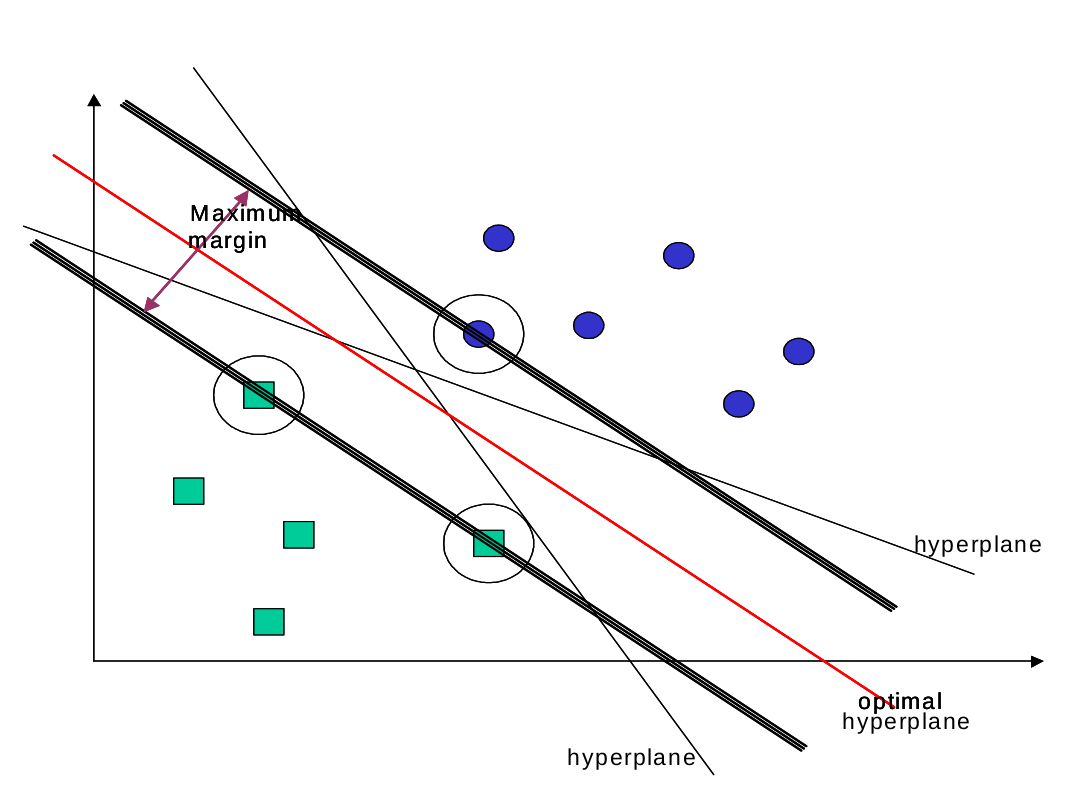
\includegraphics[width=450px]{./assets/img/svmmargin.png}
	\caption{Example of a linear seperated SVM}
	\label{fig:svmmargin}
\end{figure}

The fact that the SVM is determined by only the support vectors which are usually a very small subset of the training vectors, is great because it means that the speed does not significantly slow down with a larger amount of features.  However it is also realistic to imagine data that cannot be easily divided, this can be solved using soft margins that allow for misclassifications or in more complex cases the data can be mapped to a higher dimensional space to open up other options of dividing the data.  This higher dimensional space is referred to as the transformed feature space, however simple linear seperations in the higher dimensional space transform into non-linear seperations when you return back to the original space.  

If this feature space data is mapped to a Hilbert space referred to with $\Phi$, which allows for traditional euclidean space vector calculations to be extended to an infinite amount of dimensions using dot products using equations in the form of: $\Phi\left(x_i \right)\cdot\Phi\left(x_j \right)$.  This means that we can use what is called a kernel function to avoid ever having to determine the mapping to $\Phi$ and calculate the necessary results directly in the feature space instead.  A kernel function is in the form of: $K(x_{i},x_{j}) = \Phi(x_i) \cdot \Phi(x_j)$. \cite{supervisedMachineLearning}  There are many commonly used kernels, three of which will be used in this research: linear, polynomial (with degree 3), and radial basis function (Table \ref{tab:kernels}).  

\begin{table}[h]
	\centering
	\begin{tabular}{|p{1.5in}|p{4.5in}|}
	\hline
		\textbf{Kernel Function} & \textbf{Mathematical Formula}\\
	\hhline{|=|=|}
		Linear  & $K(x_{i},x_{j}) = \langle x_{i},x_{j}\rangle$ \\
	\hline
		Polynomial & $K(x_{i},x_{j}) = (\langle x_{i},x_{j}\rangle + 1)^d, d: degree$ \\
	\hline
		Radial Basis Function (RBF) & $K(x_{i},x_{j}) = \exp\left(\frac{- \parallel x_i - x_j \parallel^2}{2\sigma^2} /\right), \sigma : width\ of\ RBF\ function$ \\
	\hline
	\end{tabular}
	\caption{Kernels that will be used and their mathematical function} \cite{intrusionDetectionCostBased}
	\label{tab:kernels}
\end{table}

Once the SVM is trained using a kernel method of choice the only step left is to pass in all of the testing data and see which side of the hyperplane(s) it falls in order to classify it.  An SVM can at times get very computational intensive and can run very slow, this is often due to the choice of the kernel function as well as the parameters that influence the kernel.  For example, a linear kernel is very simple where as an RBF kernel is much more complex.  Two parameters that are worth mentioning for the SVM training process are $\gamma$ (gamma) and C.

Gamma is used in the polynomial and RBF kernels to define how much influence each training vector has on the seperating hyperplane(s).  A lower gamma value corresponds to a far influence, when gamma is too small the influence of any support vector may extend to the entire set and the end result would instead just be regions of high density being isolated from other high density areas.  On the converse if gamma is too high then the influence would only extend to the support vector itself.  The C parameter is the penalty cost assocated with misclassification, if C is low then classification is more relaxed compared to a higher C which will encourage more support vectors to be chosen and achieve a more accurate division. \cite{rbfSVMParameters}  There is no way to know what are the best values to choose for gamma and C because it depends on the dataset in question and so this must be done by doing testing.

\subsection{Current Support Vector Machine Solutions} \label{sec:SVMSolutions}

Support vector machines have also been applied to web threat detection as well but only in the lower layers of the OSI model dealing with network related attacks such as denial of service.  One such study used a cost based support vector machine to detect web attacks and was able to detect them with an overall accuracy of 99\%. \cite{intrusionDetectionCostBased}  Likewise, another study compared the usage of an SVM versus an artificial neural network and found that the SVM was much faster in comparison along with achieving a 99\% accuracy as well. \cite{intrusionDetectionNeural}  These results of these two studies show that the SVM approach is a viable one and can be used for practical applications with detection web threats, so it will be interesting to see how well the algorithm performs for application layer attacks as well as how it compares to the genetic algorithm approach.


